\epi{我对外科手术般进入我的身体总是有恐惧。你知道我说的是什么。}{\textit{eXistenZ}\\\textsc{TED PIKUL}}
\noindent{}
\gomarginpar{下面的内容来自 \cite{go_interfaces}。是 Ian Lance Taylor 编写的,他是 Go 的作者之一。}
在 Go 中,保留字 \first{\emph{interface}}{interface} 被赋予了多种不同的含义。
每个类型都有接口,意味着对那个类型\emph{定义了方法集合}
\index{interface!set of methods}。这段代码定义了具有一个字段和两个方法的结构类型 \type{S}。
\begin{lstlisting}[caption=定义结构和结构的方法,label=src:interface object]
type S struct { i int }
func (p *S) Get() int { return p.i }
func (p *S) Put(v int) { p.i = v }
\end{lstlisting}
也可以定义\first{接口类型}{interface!type},仅仅是方法的集合。
这里定义了一个有两个方法的接口 \type{I}:
\begin{lstlisting}
type I interface {
  Get() int
  Put(int)
}
\end{lstlisting}
\begin{lbar}
接口类型就是方法的集合。
\end{lbar}

\noindent对于接口 \type{I},\type{S} 是合法的\emph{实现},因为它定义了 \type{I}
所需的两个方法。注意,即便是没有明确定义 \type{S} 实现了 \type{I},这也是正确的。

Go 程序可以利用这个特点来实现接口的另一个含义,就是
\first{接口值}{interface!value}:

\begin{lstlisting}
func f(p I) {  |\longremark{定义一个函数接受一个接口类型作为参数;}|
    fmt.Println(p.Get()) |\longremark{\var{p} 实现了接口 \type{I},\emph{必须}有 \func{Get()} 方法;}|
    p.Put(1) |\longremark{\func{Put()} 方法是类似的。}|
}
\end{lstlisting}
\showremarks
这里的变量 \var{p} 保存了接口类型的值。因为
\type{S} 实现了 \type{I},可以调用 \func{f} 向其传递 \type{S} 类型的值的指针:
\begin{lstlisting}
var s S; f(&s)
\end{lstlisting}

获取 \type{s} 的地址,而不是 \type{S} 的值的原因,是因为在 \type{s} 
的指针上定义了方法,参阅上面的代码 \ref{src:interface object}。
这并不是必须的——可以定义让方法接受值——但是这样的话 \func{Put} 方法就不会像期望的那样工作了。

实际上,无须明确一个类型是否实现了一个接口意味着 Go 实现了叫做
\first{duck typing}{duck typing}\cite{duck_typing} 的模式。
这不是纯粹的 duck typing,因为如果可能的话 Go 编译器将对类型是否实现了接口进行实现静态检查。
然而,Go 确实有纯粹动态的方面,如可将一个接口类型转换到另一个。
通常情况下,转换的检查是在运行时进行的。
如果是非法转换——当在已有接口值中存储的类型值不匹配将要转换到的接口——程序会抛出运行时错误。

在 Go 中的接口有着与许多其他编程语言类似的思路:
C++ 中的纯抽象虚基类,Haskell 中的 typeclasses 或者 Python 中的 duck typing。
然而没有其他任何一个语言联合了接口值、静态类型检查、运行时动态转换,以及无须明确定义类型适配一个接口。
这些给 Go 带来的结果是,强大、灵活、高效和容易编写的。

\subsection{到底是什么?}
来定义另外一个类型同样实现了接口 \type{I}:
\begin{lstlisting}[caption=实现了 I 的另一个类型]
type R struct { i int }
func (p *R) Get() int { return p.i }
func (p *R) Put(v int) { p.i = v }
\end{lstlisting}
函数 \func{f} 现在可以接受 \type{R} 个 \type{S} 类型的变量。
假设需要在函数 \func{f} 中知道实际的类型。在 Go 中可以使用
 \first{type switch}{type switch} 得到。

\begin{lstlisting}
func f(p I) {
    switch t := p.(type) { |\longremark{类型判断。在 \key{switch} 语句中使用 \key{(type)}。保存类型到变量 \var{t};}|
        case *S: |\longremark{\var{p} 的实际类型是 \type{S} 的指针;}|
        case *R: |\longremark{\var{p} 的实际类型是 \type{R} 的指针;}|
        case S:  |\longremark{\var{p} 的实际类型是 \type{S};}|
        case R:  |\longremark{\var{p} 的实际类型是 \type{R};}|
        default: |\longremark{实现了 \type{I} 的其他类型。}|
    }
}
\end{lstlisting}
\showremarks
注意,得到接口变量的类型的唯一方法是使用类型判断。
在 \key{switch} 外使用 \key{(type)} 是非法的。

\subsection{空接口}
由于每个类型都能匹配到空接口:
\type{interface\{\}}。我们可以创建一个接受空接口作为参数的普通函数:
\begin{lstlisting}[caption=空接口参数的函数t,label=src:interface empty]
func g(any interface{}) int { 
    return any.(I).Get() 
}
\end{lstlisting}
在这个函数中的 \lstinline{return any.(I).Get()} 是有一点窍门的。
值 \var{any} 具有类型 \type{interface\{\}},这意味着方法没有任何约束:
它能包含任何类型。\lstinline{.(I)} 是 \first{类型断言}{type assertion},用于转换 \var{any} 到
\type{I} 类型的接口。如果有这个类型,则可以调用 \func{Get()} 函数。
因此,如果创建一个 \type{*S} 类型的新变量,也可以调用 \func{g()},
因为 \type{*S} 同样实现了空接口。
\begin{lstlisting}
s = new(S)
fmt.Println(g(s));
\end{lstlisting}
调用 \func{g} 的运行不会出问题,并且将打印 0。如果调用 \func{g()} 的参数没有实现 \type{I} 
会带来一个麻烦:
\begin{lstlisting}[caption=接口实现异常,label=src:interface fail]
i := 5		|\coderemark{声明 i 是一个"该死的" \texttt{int}}|
fmt.Println(g(i))
\end{lstlisting}
这能通过编译,但是当运行的时候会得到:

\noindent\error{panic: interface conversion: int is not main.I: missing
method Get}

\noindent{}这是绝对没问题,内建类型 \type{int} 没有 \func{Get()} 方法。

\subsection{检查接口}
在代码中,希望避免这类错误,Go 提供了检查一个变量是否实现了某个接口的方法,
同样使用了类型断言,但是这回是在 \key{if} 语句中。

\begin{lstlisting}
if ok := any.(I); ok { 
   /* 对于实现接口 I 的任意操作 */
} 
\end{lstlisting}

\section{方法}
方法就是有接收者的函数(参阅第 \ref{chap:functions} 章)。

可以在任意类型上定义方法(除了非本地类型,包括内建类型:\type{int} 类型不能有方法)。
然而可以新建一个拥有方法的整数类型。例如:
\begin{lstlisting}
type Foo int

func (self Foo) Emit() {
  fmt.Printf("%v", self)
}

type Emitter interface {
  Emit()
}
\end{lstlisting}
对那些非本地(定义在其他包的)类型也一样:
% Empty line here is critical, otherwise no new paragraph is created

\begin{minipage}{.5\textwidth}
\begin{lstlisting}[linewidth=.7\textwidth,caption=扩展内建类型错误]
func (i int) Emit() {
  fmt.Printf("%d", i)
}
\end{lstlisting}
\noindent\error{不能定义新的方法\\ 在非本地类型 int 上}
\end{minipage}
\begin{minipage}{.5\textwidth}
\begin{lstlisting}[caption=扩展非本地类型错误]
func (a *net.AddrError) Emit() {
  fmt.Printf("%v", a)
}
\end{lstlisting}
\noindent\error{不能定义新的方法\\ 在非本地类型 net.AddrError 上}
\end{minipage}

\paragraph{}  %% needed otherwise the minipage flows over

\subsection{接口类型的方法}
接口定义为一个方法的集合。方法包含实际的代码。
换句话说,一个接口就是定义,而方法就是实现。
因此,接收者不能定义为接口类型,这样做的话会引起
\error{invalid receiver type ...} 的编译器错误。来自语言说明书 \cite{go_spec} 的权威内容:
\begin{quote}
接收者类型必须是 \type{T} 或 \type{*T},这里的 \type{T} 是类型名。
\type{T} 叫做接收者基础类型或简称基础类型。基础类型一定不能使指针或接口类型,
并且定义在与方法相同的包中。
\end{quote}

\subsection{接口指针}
在 Go 中创建指向接口的指针是无意义的。
\todo{接口不是指针,不是引用类型}
\gomarginpar{Go \gorelease{2010-10-13}.} 实际上创建指向接口值的指针是非法的。
发布日志中的描述使得没有任何余地怀疑这个:
\begin{quote}
语言的改变是使用指针指向接口值不再自动反引用指针。指向接口值的指针通常是低级的错误,而不是正确的代码。
\end{quote}
这来自 \cite{go_faq}。如果不是这个限制,这个代码:
\begin{lstlisting}
var buf bytes.Buffer
io.Copy(buf, os.Stdin)
\end{lstlisting}
就会复制标准输入到 \var{buf} 的副本,而不是 \var{buf} 本身。
这看起来永远不会是一个期望的结果。

\section{接口名字}
根据规则,单方法接口命名为方法名加上 \emph{-er} 后缀:Read\emph{er},Writ\emph{er},Formatt\emph{er} 等。

有一堆这样的命名,高效的反映了它们职责和包含的函数名。
\func{Read},\func{Write},\func{Close},\func{Flush},\func{String} 等等有着规范的声明和含义。
为了避免混淆,除非有类似的声明和含义,否则不要让方法与这些重名。
相反的,如果类型实现了与众所周知的类型相同的方法,那么就用相同的名字和声明;
将字符串转换方法命名为 \func{String} 而不是 \func{ToString}。
\gomarginpar{文本复制于 \cite{effective_go}。}

\section{简短的例子}
\label{sec:a sorting example}
回顾那个冒泡排序的练习(Q\ref{ex:bubble}),对整型数组排序:
\begin{lstlisting}
func bubblesort(n []int) {
    for i := 0; i < len(n)-1; i++ {
	for j := i + 1; j < len(n); j++ {
	    if n[j] < n[i] {
		    n[i], n[j] = n[j], n[i]
	    }
	}
    }
}
\end{lstlisting}
排序字符串的版本是类似的,除了函数的声明:
\begin{lstlisting}
func bubblesortString(n []string) { /* ... */ }
\end{lstlisting}
基于此,可能会需要两个函数,每个类型一个。而通过使用接口可以让这个变得更加通用 \index{generic}。

来创建一个可以对字符串和整数进行排序的函数,这个例子的某些行是无法运行的:
\begin{lstlisting}
func sort(i []interface{}) { |\longremark{函数将接收一个空接口的 slice;}|
    switch i.(type) {        |\longremark{使用 type switch 找到输入参数实际的类型;}|
	case string:         |\longremark{然后排序;}|
	    // ...
	case int:
	    // ...
    }
    |\longremark{返回排序的 slice。}|
}
\end{lstlisting}
\showremarks
但是如果用 \lstinline|sort([]int{1, 4, 5})| 调用这个函数,会失败:
\error{cannot use i (type []int) as type []interface { } in function argument}

这是因为 Go 不能简单的将其转换为接口的 \emph{slice}。
转换到接口是容易的,但是转换到 slice 的开销就高了。

简单来说
\gomarginpar{关于这个话题完整的邮件列表讨论可以在 \cite{go_nuts_interfaces} 这里找到。}
:Go 不能(隐式)转换为 slice。

那么如何创建 Go 形式的这些“通用”函数呢?
用 Go 隐式的处理来代替 type switch 方式的类型推断吧。
下面的步骤是必须的:
\begin{enumerate}
\item 定义一个有着若干排序相关的方法的接口类型(这里叫做 \type{Sorter})。
至少需要获取 slice 长度的函数,比较两个值的函数和交换函数;
\begin{lstlisting}
type Sorter interface {
    Len() int           |\coderemark{\texttt{len()} 作为方法}|
    Less(i, j int) bool |\coderemark{\texttt{p[j] $<$ p[i]} 作为方法}|
    Swap(i, j int)      |\coderemark{\texttt{p[i], p[j] = p[j], p[i]} 作为方法}|
}
\end{lstlisting}
\item 定义用于排序 slice 的新类型。注意定义的是 slice 类型;
\begin{lstlisting}
type Xi []int
type Xs []string
\end{lstlisting}
\item 实现 \type{Sorter} 接口的方法。
整数的:
\begin{lstlisting}
func (p Xi) Len() int               { return len(p) }
func (p Xi) Less(i int, j int) bool { return p[j] < p[i] }
func (p Xi) Swap(i int, j int)      { p[i], p[j] = p[j], p[i] }
\end{lstlisting}
和字符串的:
\begin{lstlisting}
func (p Xs) Len() int               { return len(p) }
func (p Xs) Less(i int, j int) bool { return p[j] < p[i] }
func (p Xs) Swap(i int, j int)      { p[i], p[j] = p[j], p[i] }
\end{lstlisting}
\item 编写作用于 \type{Sorter} 接口的\emph{通用}排序函数。
\begin{lstlisting}
func Sort(x Sorter) { |\longremark{\var{x} 现在是 \texttt{Sorter} 类型;}|
    for i := 0; i < x.Len() - 1; i++ { |\longremark{使用定义的函数,实现了冒泡排序。}|
	for j := i + 1; j < x.Len(); j++ {
	    if x.Less(i, j) {
		x.Swap(i, j)
	    }
	}
    }
}
\end{lstlisting}
\showremarks
\end{enumerate}
现在可以像下面这样使用通用的 \func{Sort} 函数:
\begin{lstlisting}
ints := Xi{44, 67, 3, 17, 89, 10, 73, 9, 14, 8}
strings := Xs{"nut", "ape", "elephant", "zoo", "go"}

Sort(ints)
fmt.Printf("%v\n", ints)
Sort(strings)
fmt.Printf("%v\n", strings)
\end{lstlisting}

\section{自省}
\label{sec:introspection}
在程序中,可以用 \key{switch} 了解接口变量的动态类型。
例如类型断言\gomarginindex{类型断言}{type assertion}使用了在圆括号里的关键字
\key{type} 实现了类型断言的语法。在 switch 中定义的变量表达式,每个分支都对应变量的相应类型。
\begin{lstlisting}[caption=动态的找到类型]
package main
type PersonAge struct { |\longremark{首先定义两个结构作为新类型,\texttt{PersonAge};}|
	name string
	age  int
}

type PersonShoe struct { |\longremark{和 \texttt{PersonShoe};}|
	name     string
	shoesize int
}

func main() {
	p1 := new(PersonAge)
	p2 := new(PersonShoe)
	WhichOne(p1)
	WhichOne(p2)
}

func WhichOne(x interface{}) { |\longremark{这个函数必须能接收\emph{两种}类型作为输入,%
因此使用每个类型都实现了的空接口;}|
	switch t := x.(type) { |\longremark{type switch:\texttt{(type)};}|
	case *PersonAge:	|\longremark{当用 \func{new} 分配了内存,这就是个指针。%
因此检查是否为 \type{*PersonAge}。如果 \func{WhichOne()} 被非指针类型调用,则应当检查 \type{PersonAge}。}|
		println("Age person")
	case *PersonShoe:
		println("Shoe person")
	}
}
\end{lstlisting}
\showremarks

下面有另外一个例子展示,不过这回检查了更多的(内建)类型:
\begin{lstlisting}[caption=更普通的 type switch]
switch t := interfaceValue.(type) { |\coderemark{type switch}|
case bool:
    fmt.Printf("boolean %t\n", t)
case int:
    fmt.Printf("integer %d\n", t)
case *bool:
    fmt.Printf("pointer to boolean %t\n", *t)
case *int:
    fmt.Printf("pointer to integer %d\n", *t)
default:
    fmt.Printf("unexpected type %T", t)  // \%T prints type
}
\end{lstlisting}

\subsection{自省和反射}
\label{subsec:introspection and reflection}
在下面的例子中,了解一下定义在 \type{Person} 的定义中的 “标签”(这里命名为“namestr”)。
为了做到这个,需要 \package{reflect}\index{package!reflect} 包(在 Go 中没有其他方法)。
要记得,查看标签意味着返回\emph{类型}的定义。因此使用 \package{reflect} 包来指出变量的类型,
\emph{然后}访问标签。
\begin{lstlisting}[caption=Introspection using reflection,label=src:introspection]
|\begin{tikzpicture}[overlay]
\draw [->,thick] (2.8,-6.00) node [left] %
{\longremark{We are dealing with a \type{PtrValue} and according %
to the documentation\footnote{\texttt{godoc reflect}}:%
\begin{quote} %
\texttt{\func{func} (v *PtrValue) Elem() Value}\\%
Elem returns the value that v points to. %
If v is a nil pointer, Elem returns a nil Value. %
\end{quote} %
we can use \func{Elem()} to get the type the pointer points to. %
In this case \type{*reflect.StructValue};}} %
to (2.8,-5.20);
%
\draw [->,thick] (3.8,-6.00) node [left] %
{\longremark{\func{Type()} returns \type{reflect.Type};}} %
to (3.8,-5.20);
\draw [->,thick] (5.4,-6.00) node [left] %
{\longremark{%
Again according to the documentation, we have:\\%
\begin{quote} %
\ldots which returns an object with interface %
type \type{Type}.  That contains a pointer to a struct of type %
\type{*StructType}, %
\type{*IntType}, etc. representing the details of the underlying type. %
A type switch or type assertion can reveal which. %
\end{quote} %
So we can access your specific type as a member of this struct. Which %
we do with \type{(*reflect.StructType)};}} %
to (5.4,-5.20);
%
\draw [->,thick] (6.8,-6.00) node [left] %
{\longremark{%
A \type{StructType} has a number of methods, one of which is %
\func{Field($n$)} which returns the $n^{th}$ field of a structure. %
The type of this return is a \type{StructField}; %
}} %
to (6.8,-5.20);
%
\draw [->,thick] (8.4,-6.00) node [left] %
{\longremark{We finally have the type we are after. Now we can use the %
methods defined for \type{*StructType}, like \func{Field(n)}, which %
returns the n$^{th}$ field of our struct as a \type{StructField};}} %
to (8.4,-5.20);
%
\draw [->,thick] (9.4,-6.00) node [left] %
{\longremark{The struct \type{StructField} has a \var{Tag} member which %
returns the tag-name as a string. So on the $0^{th}$ field we can %
unleash \func{.Tag} to access this name: \texttt{Field(0).Tag}. This %
\emph{finally} gives us \texttt{namestr}.}}%
to (9.4,-5.20);
\end{tikzpicture}|
type Person {
    name string "namestr"
    age  int
}

p1 := new(Person)   |\coderemark{\func{new} returns a pointer to Person}|
ShowTag(p1)	    |\coderemark{\func{ShowTag()} is now called with this pointer}|

func ShowTag(i interface{}) {
    switch t := reflect.NewValue(i).(type) { |\coderemark{Type assertion}|
    case *reflect.PtrValue:		     |\coderemark{\var{p1} is a pointer}|
	tag := t.Elem().Type().(||*reflect.StructType).Field(0).Tag
||
\end{lstlisting}

\showremarks

%% look at layout
为了让类型和值之间的区别更加清晰,看下面的代码:
\begin{lstlisting}[caption=反射类型和值]
func show(i interface{}) {
    switch t := i.(type) {
      case *Person:
        r := reflect.NewValue(i) |\coderemark{进入反射的世界}|
	tag := |\longremark{这里希望获得“标签”,意味着转向类型。%
因此需要\newline\lstinline{Elem().Type().(*reflect.StructType)} 来获取它;}|
	  r.(*reflect.PtrValue).Elem().Type().(*reflect.StructType).Field(0).tag
	nam := |\longremark{现在希望访问其中一个成员的\emph{值},%
使用\newline\lstinline{Elem().(*reflect.StructValue)} 获取它。%
现在了解到了结构。然后访问了第一个字段 \lstinline{Field(0)},告诉 \package{reflect} 是%
\var{*reflect.StringValue} 并且调用了其中的 \lstinline{Get()} 方法。 %
\begin{figure}[H] %
\hskip3\baselineskip\parbox{0.7\textwidth}{\caption[使用反射去除层次关系]{用反射去除层次关系。%
通过 \mbox{\type{*reflect.PtrValue}} 访问 \type{*Person},使用 \prog{godoc reflect} 中描述的方法%
获得 \type{string} 内部包含的内容。}} %
\label{fig:reflection} %
\begin{center} %
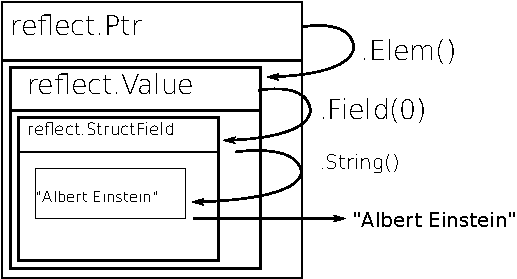
\includegraphics[scale=0.75]{fig/reflection.pdf} %
\end{center}\end{figure} %
在反射的世界里,当使用 \type{Value} 时,反射就会将层次关系去除。}|
	  r.(*reflect.PtrValue).Elem().(*reflect.StructValue).Field(0).|\newline|(*reflect.StringValue).Get()
    }
}
\end{lstlisting}
\showremarks

设置值与获得值类似,但是仅仅工作在\emph{可导出}的成员上。这些代码:

\begin{minipage}{.5\textwidth}
\begin{lstlisting}[caption=私有成员的反射]
type Person struct {
 name string "namestr"
 age  int
}

func Set(i interface{}) {
 switch t := i.(type) {
 case *Person:
  r := reflect.NewValue(i)
  r.(*reflect.PtrValue).Elem().
    (*reflect.StructValue).
    FieldByName("name").
    (*reflect.StringValue).
    Set("Albert Einstein")
  }
}
\end{lstlisting}
\end{minipage}
\hspace{2em}
\begin{minipage}{.5\textwidth}
\begin{lstlisting}[caption=公有成员的反射]
type Person struct {
 Name string "namestr" |\coderemark{}|
 age  int
}

func Set(i interface{}) {
 switch t := i.(type) {
 case *Person:
  r := reflect.NewValue(i)
  r.(*reflect.PtrValue).Elem().
   (*reflect.StructValue).
   FieldByName("Name"). |\coderemark{}|
   (*reflect.StringValue).
   Set("Albert Einstein")
  }
}
\end{lstlisting}
\end{minipage}
左边的代码可以编译并运行,但是当运行的时候,将得到打印了栈的\emph{运行时}错误:

\noindent\error{panic: cannot set value obtained via unexported struct
field}

\noindent{}右边的代码没有问题,并且设置了成员变量 \var{Name} 
为"Albert Einstein"。当然,这仅仅工作于调用 \func{Set()} 时传递一个指针参数。

\section{练习}
\begin{Exercise}[title={接口和编译},difficulty=1]
\Question
在第 \pageref{src:interface fail} 页的代码 \ref{src:interface fail} 
编译正常——就像文中开始描述的那样。但是当运行的时候,会得到运行时错误,
因此有些东西\emph{有}错误。为什么代码编译没有问题呢?
\end{Exercise}

\begin{Answer}
\Question
代码能够编译是因为整数类型实现了空接口,这是在编译时检查的。

修复这个正确的途径是测试这个空接口可以被转换,如果可以,调用对应的方法。
\ref{src:interface empty} 列出的 Go 代码中定义了函数 \func{g}——这里重复一下:
\begin{lstlisting}
func g(any interface{}) int { return any.(I).Get() }
\end{lstlisting}

\noindent{}应当修改为:
\begin{lstlisting}
func g(any interface{}) int {
    if v, ok := any.(I); ok {	// 检查是否可以转换
	return v.Get()		// 如果可以,调用 Get()
    }
    return -1			// 随便返回个什么
}
\end{lstlisting}
如果现在调用 \func{g()},就不会有运行时错误了。在 Go 中这种用法被称作``comma ok''。
\end{Answer}


\begin{Exercise}[title={Pointers and reflection},difficulty=5]
\label{ex:pointers and reflection}
\Question
One of the last paragraphs in section "\titleref{subsec:introspection and reflection}" 
on page \pageref{subsec:introspection and reflection}, has
the following words:
\begin{quote}
The code on the right works OK and sets the member \var{Name}
to "Albert Einstein". Of course this only works when you call \func{Set()}
with a pointer argument.
\end{quote}
Why is this the case?
\end{Exercise}

\begin{Answer}
\Question
When called with a non-pointer argument the variable is a copy (call-by-value). So you
are doing the reflection voodoo on a copy. And thus you are \emph{not}
changing the original value, but only this copy.
\end{Answer}


\begin{Exercise}[title={接口和最大最小},difficulty=1]
\Question
构造一个通用的最大最小,使得可以同时工作于整数和字符串,就像第 \titleref{sec:a sorting example} 节中那样。
\end{Exercise}

\begin{Answer}
\Question
\end{Answer}


\cleardoublepage
\section{答案}
\shipoutAnswer
